%----------------------------------------------
%      CHAPTER
%----------------------------------------------
\chapter{Development of the Baseline Vehicles}\label{chapter:baseline-vehicles}

Three of the most productive \gls{hcv} configurations were selected as baselines. A report from the compiled by Nordengen for the \gls{oecd} highlighted that the following combinations were the four most common articulated truck configurations in South Africa \cite{Nordengen2008}:

\begin{enumerate}
	\item A 6x4 truck-tractor hauling a 3-axle semi-trailer
	\item A 6x4 truck-tractor hauling two 2-axle semi-trailers connected with fifth-wheel couplings
	\item A 6x4 truck-tractor hauling a 2-axle semi-trailer
	\item A 6x4 truck-tractor hauling a tridem semi-trailer leader and tandem semi-trailer follower connected with fifth-wheel couplings
\end{enumerate}

Illustrations of each of the workhorse combinations are included in Figure \ref{figure:OECD workhorse combinations}.

%----------------------------------------------
%      FIGURE
%----------------------------------------------
\begin{figure*}[ht!]
	\centering
	\begin{subfigure}[t]{0.45\textwidth}
		\centering
		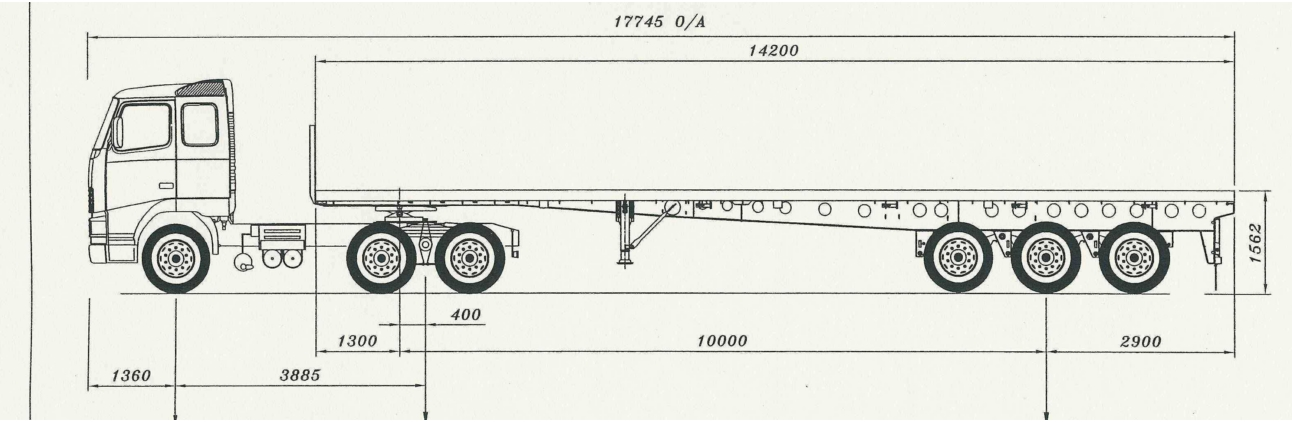
\includegraphics[height=1.0in]{fig/oecd_workhorse-combination_1}
		\caption{Workhorse 1}
	\end{subfigure}%
	\hfill
	\begin{subfigure}[t]{0.45\textwidth}
		\centering
		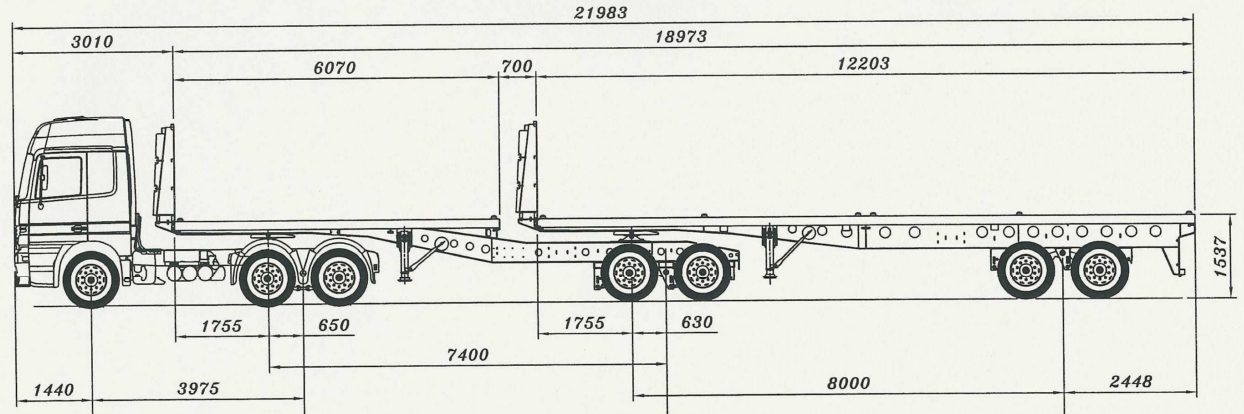
\includegraphics[height=1.0in]{fig/oecd_workhorse-combination_2}
		\caption{Workhorse 2}
	\end{subfigure}

	\begin{subfigure}[t]{0.45\textwidth}
		\centering
		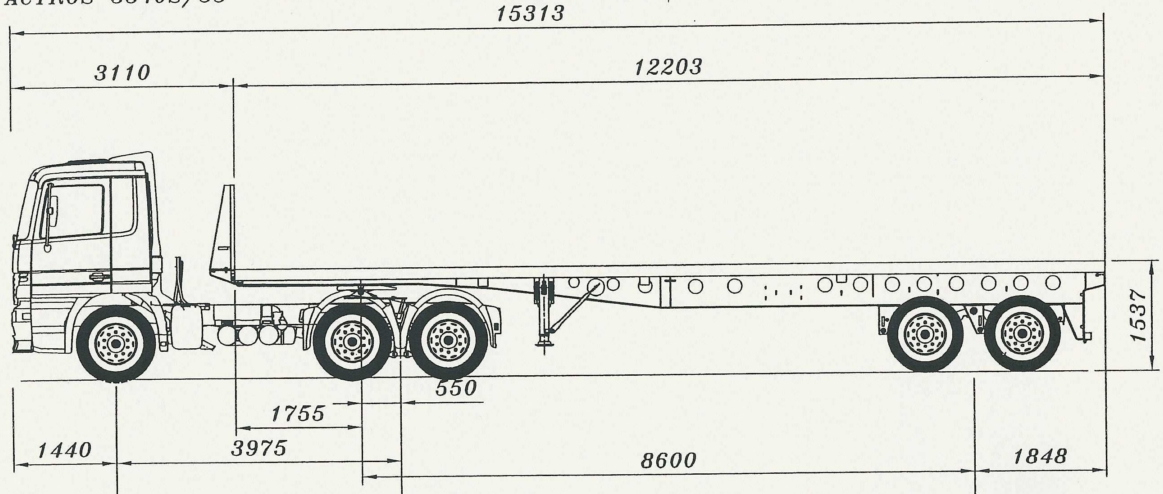
\includegraphics[height=1.0in]{fig/oecd_workhorse-combination_3}
		\caption{Workhorse 3}
	\end{subfigure}
	\hfill
	\begin{subfigure}[t]{0.45\textwidth}
		\centering
		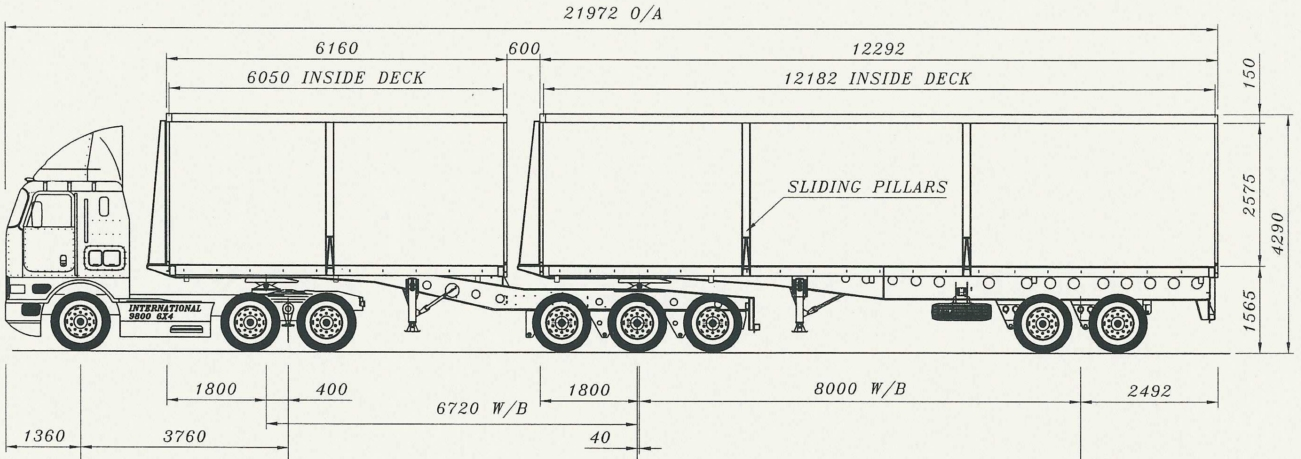
\includegraphics[height=1.0in]{fig/oecd_workhorse-combination_4}
		\caption{Workhorse 4}
	\end{subfigure}
	\caption{OECD workhorse combinations}
	\label{figure:OECD workhorse combinations}
\end{figure*}
%----------------------------------------------
%      FIGURE
%----------------------------------------------

These four workhorse vehicles have during the \gls{pbs} pilot project in South Africa been replaced by two more productive \gls{pbs} equivalents which were chosen as the first two baseline combinations:

\begin{enumerate}
	\item A 6x4 truck-tractor hauling a quad-axle semi-trailer
	\item A 6x4 truck-tractor hauling a set of tridem semi-trailers
\end{enumerate}

As of 2016 a rigid drawbar combination (known as a truck and dog combination in Australia) was still the single biggest category of vehicles approved via \gls{pbs} as can be seen in Figure \ref{figure:distribution-of-australian-pbs-fleet} \cite{Grote2017}. These combinations are not very prevalent in South Africa outside of the forestry industry, however it is envisioned that as the pilot project progresses in South Africa and \gls{pbs} becomes more widely adopted, that this combination will become widely-used.

%----------------------------------------------
%      FIGURE
%----------------------------------------------
\begin{figure}[H]
	\centering
	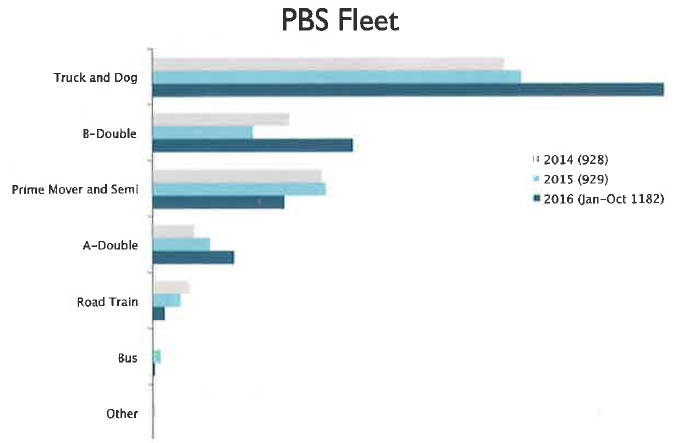
\includegraphics[width=1\textwidth]{fig/globaltrailermag_truck-and-dog-pbs-fleet-australia}
	\caption{Distribution of the Australian PBS fleet as of Oct 2016 \cite{Grote2017}}
	\label{figure:distribution-of-australian-pbs-fleet}
\end{figure}
%----------------------------------------------
%      FIGURE
%----------------------------------------------

%----------------------------------------------
%      SECTION
%----------------------------------------------
\section{Design Parameters for the Baseline Vehicles}\label{section:baseline-vehicles-design-parameters}

The design of the mechanical properties of the baseline vehicles is beyond the scope of this dissertation. Thus, combinations matching the designs chosen for baseline vehicles that were assessed within the \gls{pbs} framework in South Africa were used as a guide to develop the baseline combinations.

The baseline combinations use the same baseline prime mover (for which data was provided by the \gls{oem}) with the geometrical properties of the prime mover (such as the wheelbase and hitch location) modified to suit the design of each baseline combination.

Representative axles were developed for the baseline combinations. The prime movers used the same set of steer and drive axles and the trailer axles differed in track width and tyre size for each trailer.

Sections~\ref{section:baseline-quad-semi}~to~\ref{section:baseline-rigid-drawbar-combination} describe the configuration of each baseline combination according to the baseline prime mover units, trailer units and axles.

%      SUBSECTION
%----------------------------------------------
\subsection{Baseline Quad Semi-trailer Combination}\label{section:baseline-quad-semi}

The quad semi-trailer fuel tanker is one of the most common quad-axle semi-trailer combinations operated in South Africa. A \gls{lpg} quad was selected as the baseline for this combination. The configuration of this baseline combination is as per Table~\ref{table:configuration-quad-semi} and a simplified \gls{ga} drawing of the combination is included in Figure \ref{figure:baseline-ga-quad-semi}.

%----------------------------------------------
%      TABLE
%----------------------------------------------
\begin{table}[H]
	\centering\footnotesize
	\begin{threeparttable}

		\begin{tabulary}{\textwidth}{llc}
			\toprule
\textbf{Vehicle unit, axle or tyre} & \textbf{Description} & \textbf{VDP Table (see Appendix~\ref{appendix:baseline-models})} \\
		\midrule
    Prime mover unit & Truck tractor & Table~\ref{table:vdp-range-prime-mover-tractor} \\
    Trailer unit & Quad semi-trailer & Table~\ref{table:vdp-range-trailer-quad-semi} \\
    Steer axle  & Steer axle with 315/80 R22.5 tyres & Table~\ref{table:vdp-range-axle-steer-315} \\
    Drive axle & Drive axle with 315/80 R22.5 tyres & Table~\ref{table:vdp-range-axle-drive-315} \\
    Trailer axle & Trailer axle with 445/65 R22.5 tyres & Table~\ref{table:vdp-range-axle-trailer-445} \\
    Steer tyre & 315/80 R22.5 (singles) & Table~\ref{table:vdp-tyre-315} \\
    Drive tyre  & 315/80 R22.5 (duals) & Table~\ref{table:vdp-tyre-315} \\
    Trailer tyre & 445/65 R22.5 (singles) & Table~\ref{table:vdp-tyre-445} \\
			\bottomrule
		\end{tabulary}

		\caption{Configuration of the baseline quad-semi combination}
		\label{table:configuration-quad-semi}

		%\begin{tablenotes}
		%\item[1] %\tnote{1}
		%\end{tablenotes}

	\end{threeparttable}
\end{table}
%----------------------------------------------
%      TABLE
%----------------------------------------------

\newpage

\newgeometry{left=5mm,right=5mm,top=5mm,bottom=10mm, footskip=0mm}

\begin{landscape}\centering
\vspace*{\fill}
%----------------------------------------------
%      FIGURE
%----------------------------------------------
\begin{figure}[H]
	\centering
	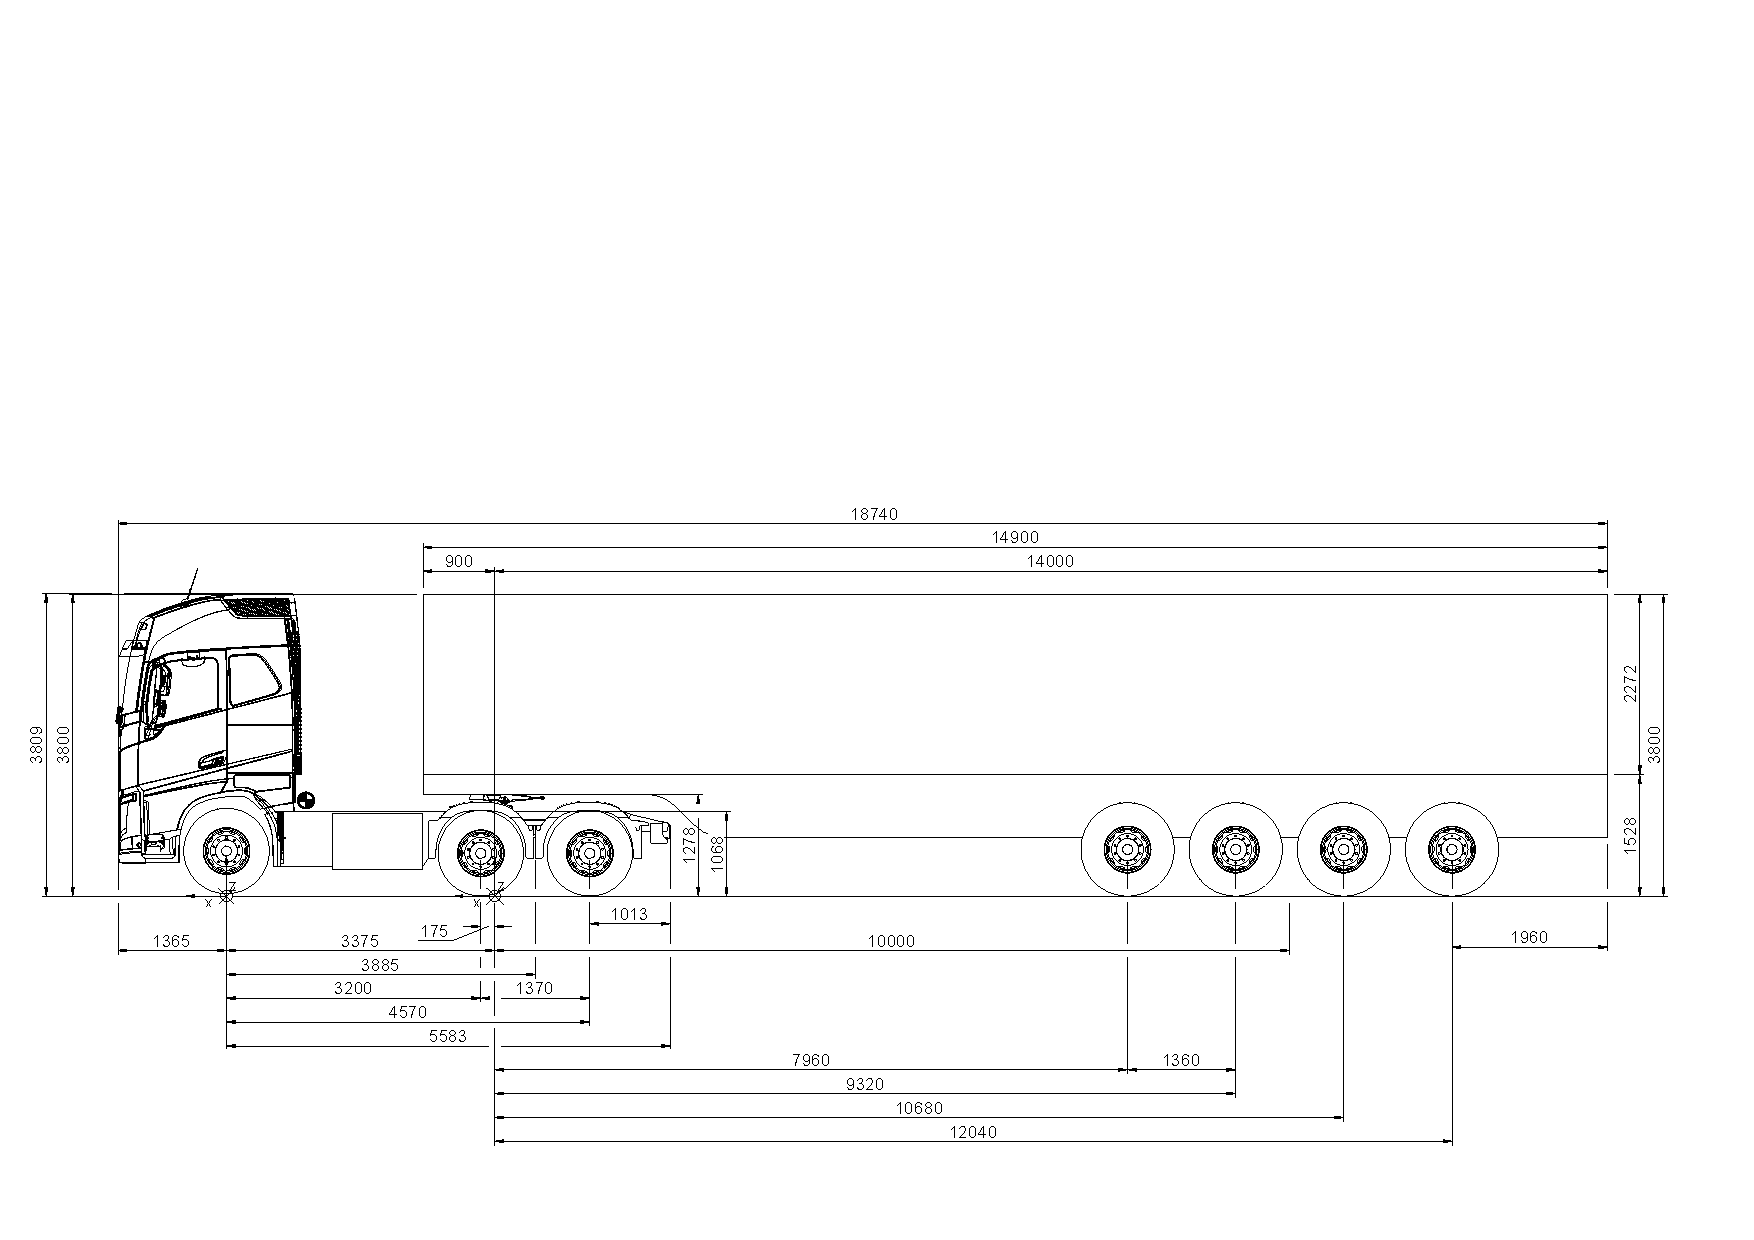
\includegraphics[width=1.3\textwidth]{fig/baseline_ga_quad-semi}
	\caption{Baseline quad semi-trailer combination GA drawing}
	\label{figure:baseline-ga-quad-semi}
\end{figure}
%----------------------------------------------
%      FIGURE
%----------------------------------------------
\vfill
\end{landscape}

\restoregeometry



%      SUBSECTION
%----------------------------------------------
\subsection{Baseline Tridem Interlink Combination}\label{section:baseline-tridem-interlink}

A tridem interlink side-tipper used for the transportation of coal ore was modelled as the baseline tridem interlink combination. The configuration of this baseline combination is as per Table~\ref{table:configuration-tridem-interlink} and a \gls{ga} drawing of the combination is included in Figure~\ref{figure:baseline-ga-tridem-interlink}.

%----------------------------------------------
%      TABLE
%----------------------------------------------
\begin{table}[H]
	\centering\footnotesize
	\begin{threeparttable}

		\begin{tabulary}{\textwidth}{llc}
			\toprule
    \textbf{Vehicle unit, axle or tyre} & \textbf{Description} & \textbf{VDP Table (see Appendix~\ref{appendix:baseline-models})} \\
    			\midrule
    Prime mover unit & Truck tractor & Table~\ref{table:vdp-range-prime-mover-tractor} \\
    Lead trailer unit & Tridem interlink leader & Table~\ref{table:vdp-range-trailer-tridem-interlink-leader} \\
    Follower trailer unit & Tridem interlink follower & Table~\ref{table:vdp-range-trailer-tridem-interlink-follower} \\
    Steer axle  & Steer axle with 315/80 R22.5 tyres & Table~\ref{table:vdp-range-axle-steer-315} \\
    Drive axle & Drive axle with 315/80 R22.5 tyres & Table~\ref{table:vdp-range-axle-drive-315} \\
    Trailer axle & Trailer axle with 315/80 R22.5 tyres & Table~\ref{table:vdp-range-axle-trailer-315} \\
    Steer tyre & 315/80 R22.5 (singles) & Table~\ref{table:vdp-tyre-315} \\
    Drive tyre  & 315/80 R22.5 (duals) & Table~\ref{table:vdp-tyre-315} \\
    Trailer tyre & 315/80 R22.5 (duals) & Table~\ref{table:vdp-tyre-315} \\
			\bottomrule
		\end{tabulary}

		\caption{Configuration of the baseline tridem interlink combination}
		\label{table:configuration-tridem-interlink}

		%\begin{tablenotes}
		%\item[1] %\tnote{1}
		%\end{tablenotes}

	\end{threeparttable}
\end{table}
%----------------------------------------------
%      TABLE
%----------------------------------------------

\newgeometry{left=5mm,right=5mm,top=5mm,bottom=10mm, footskip=0mm}

\begin{landscape}\centering
	\vspace*{\fill}
%----------------------------------------------
%      FIGURE
%----------------------------------------------
\begin{figure}[H]
	\centering
	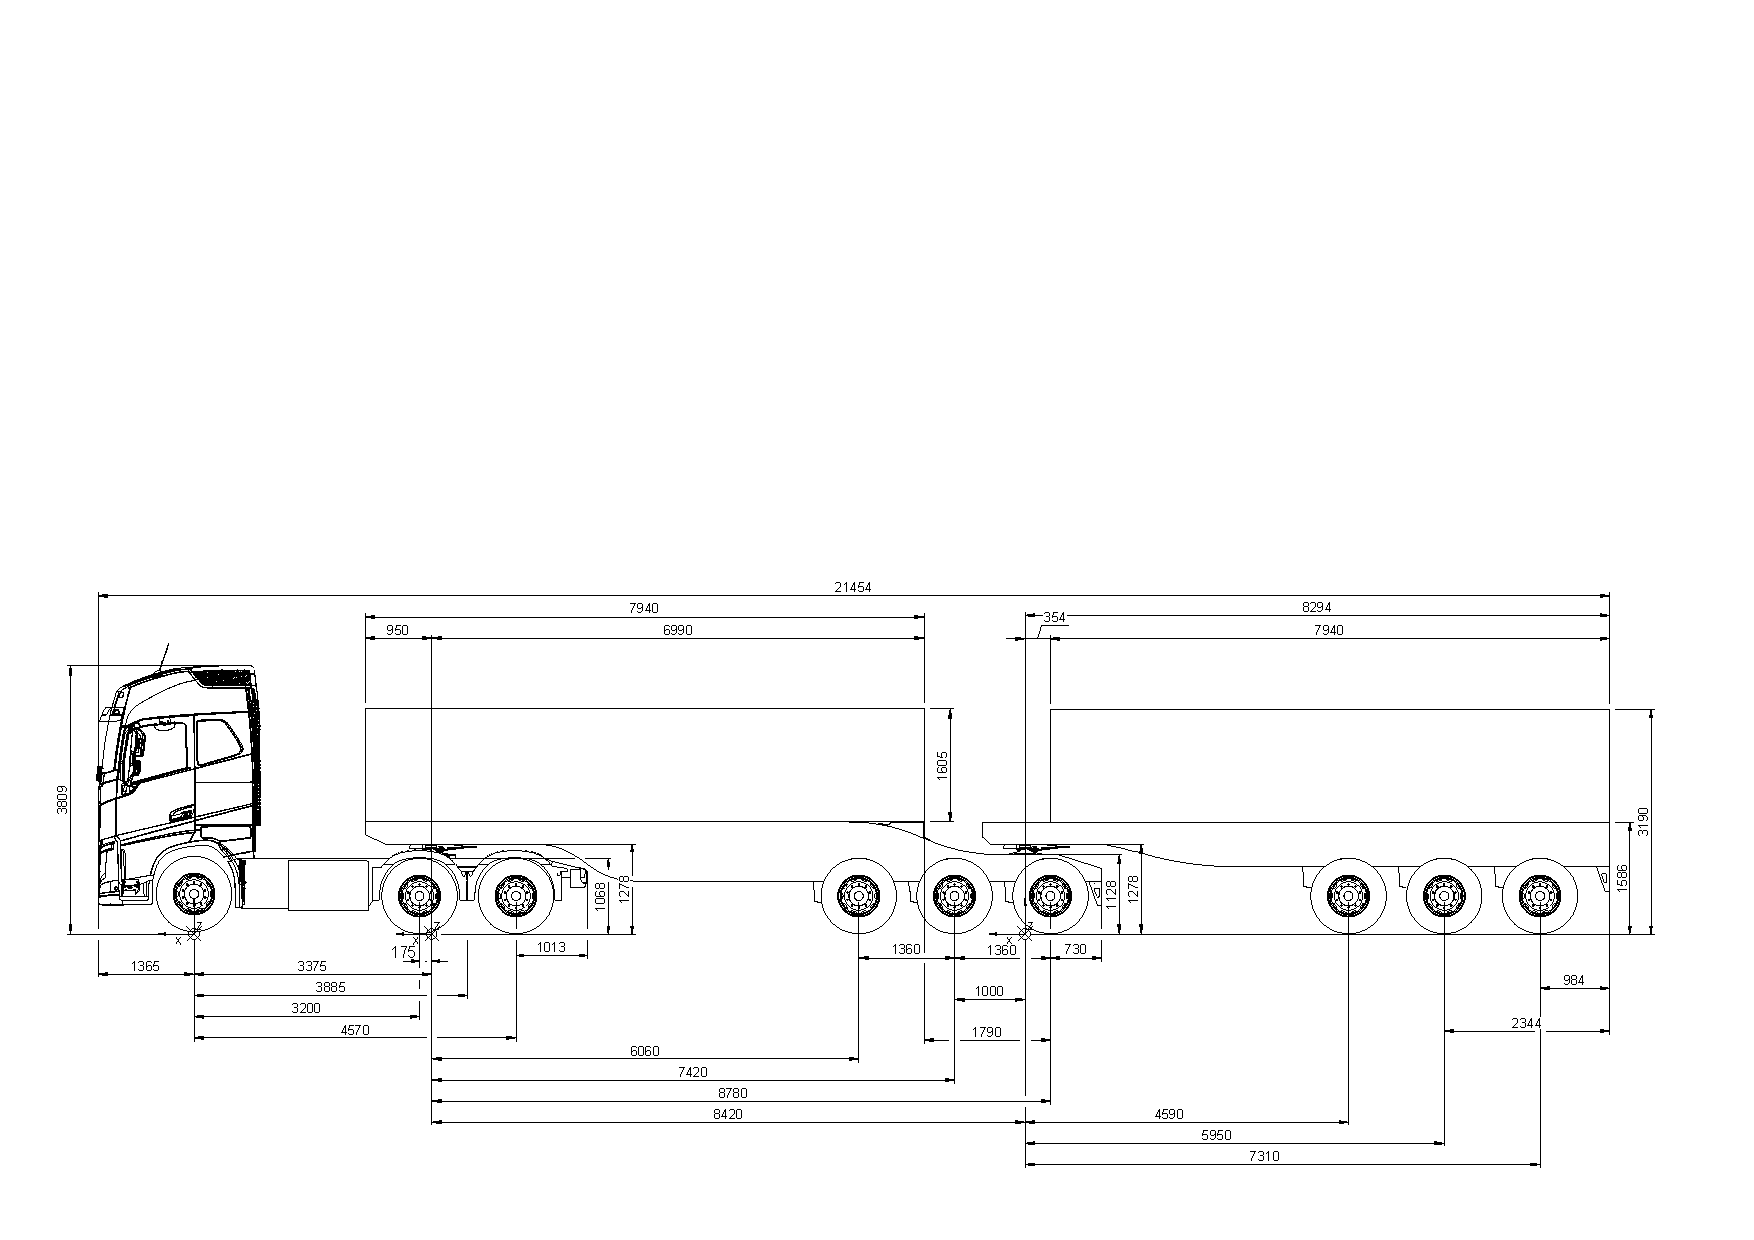
\includegraphics[width=1.3\textwidth]{fig/baseline_ga_tridem-interlink}
	\caption{Baseline tridem interlink combination GA drawing}
	\label{figure:baseline-ga-tridem-interlink}
\end{figure}
%----------------------------------------------
%      FIGURE
%----------------------------------------------
	\vfill
\end{landscape}

\restoregeometry

%      SUBSECTION
%----------------------------------------------
\subsection{Baseline Rigid Drawbar Combination}\label{section:baseline-rigid-drawbar-combination}

The rigid drawbar combination is most prevalent in South Africa in the logging industry. The baseline rigid drawbar combination was modelled from a combination intended for the transport of timber. The configuration of this baseline combination is as per Table~\ref{table:configuration-rigid-drawbar-combination} and a simplified \gls{ga} drawing of the combination is included in Figure~\ref{figure:baseline-ga-rigid-drawbar-combination}.

%----------------------------------------------
%      TABLE
%----------------------------------------------
\begin{table}[H]
	\centering\footnotesize
	\begin{threeparttable}

		\begin{tabulary}{\textwidth}{llc}
			\toprule
    \textbf{Vehicle unit, axle or tyre} & \textbf{Description} & \textbf{VDP Table (see Appendix~\ref{appendix:baseline-models})} \\
    			\midrule
    Prime mover unit & Rigid truck & Table~\ref{table:vdp-range-prime-mover-rigid} \\
    Lead trailer unit & Tridem semi-trailer & Table~\ref{table:vdp-range-trailer-rigid-combination-trailer} \\
    Dolly unit & Dolly & Table~\ref{table:vdp-range-trailer-rigid-combination-dolly} \\
    Steer axle  & Steer axle with 315/80 R22.5 tyres & Table~\ref{table:vdp-range-axle-steer-315} \\
    Drive axle & Drive axle with 315/80 R22.5 tyres & Table~\ref{table:vdp-range-axle-drive-315} \\
    Trailer axle\tnote{1} & Trailer axle with 285/70 R19.5 tyres & Table~\ref{table:vdp-range-axle-trailer-285} \\
    Steer tyre & 315/80 R22.5 (singles) & Table~\ref{table:vdp-tyre-315} \\
    Drive tyre  & 315/80 R22.5 (duals) & Table~\ref{table:vdp-tyre-315} \\
    Trailer tyre\tnote{1} & 285/70 R19.5 (duals) & Table~\ref{table:vdp-tyre-285} \\
			\bottomrule
		\end{tabulary}

		\caption{Configuration of the baseline rigid drawbar combination}
		\label{table:configuration-rigid-drawbar-combination}

		\begin{tablenotes}
		\item[1] The dolly axle is considered as a trailer axle
		\end{tablenotes}

	\end{threeparttable}
\end{table}
%----------------------------------------------
%      TABLE
%----------------------------------------------

\newgeometry{left=5mm,right=5mm,top=5mm,bottom=10mm, footskip=0mm}

\begin{landscape}\centering
	\vspace*{\fill}
%----------------------------------------------
%      FIGURE
%----------------------------------------------
\begin{figure}[H]
	\centering
	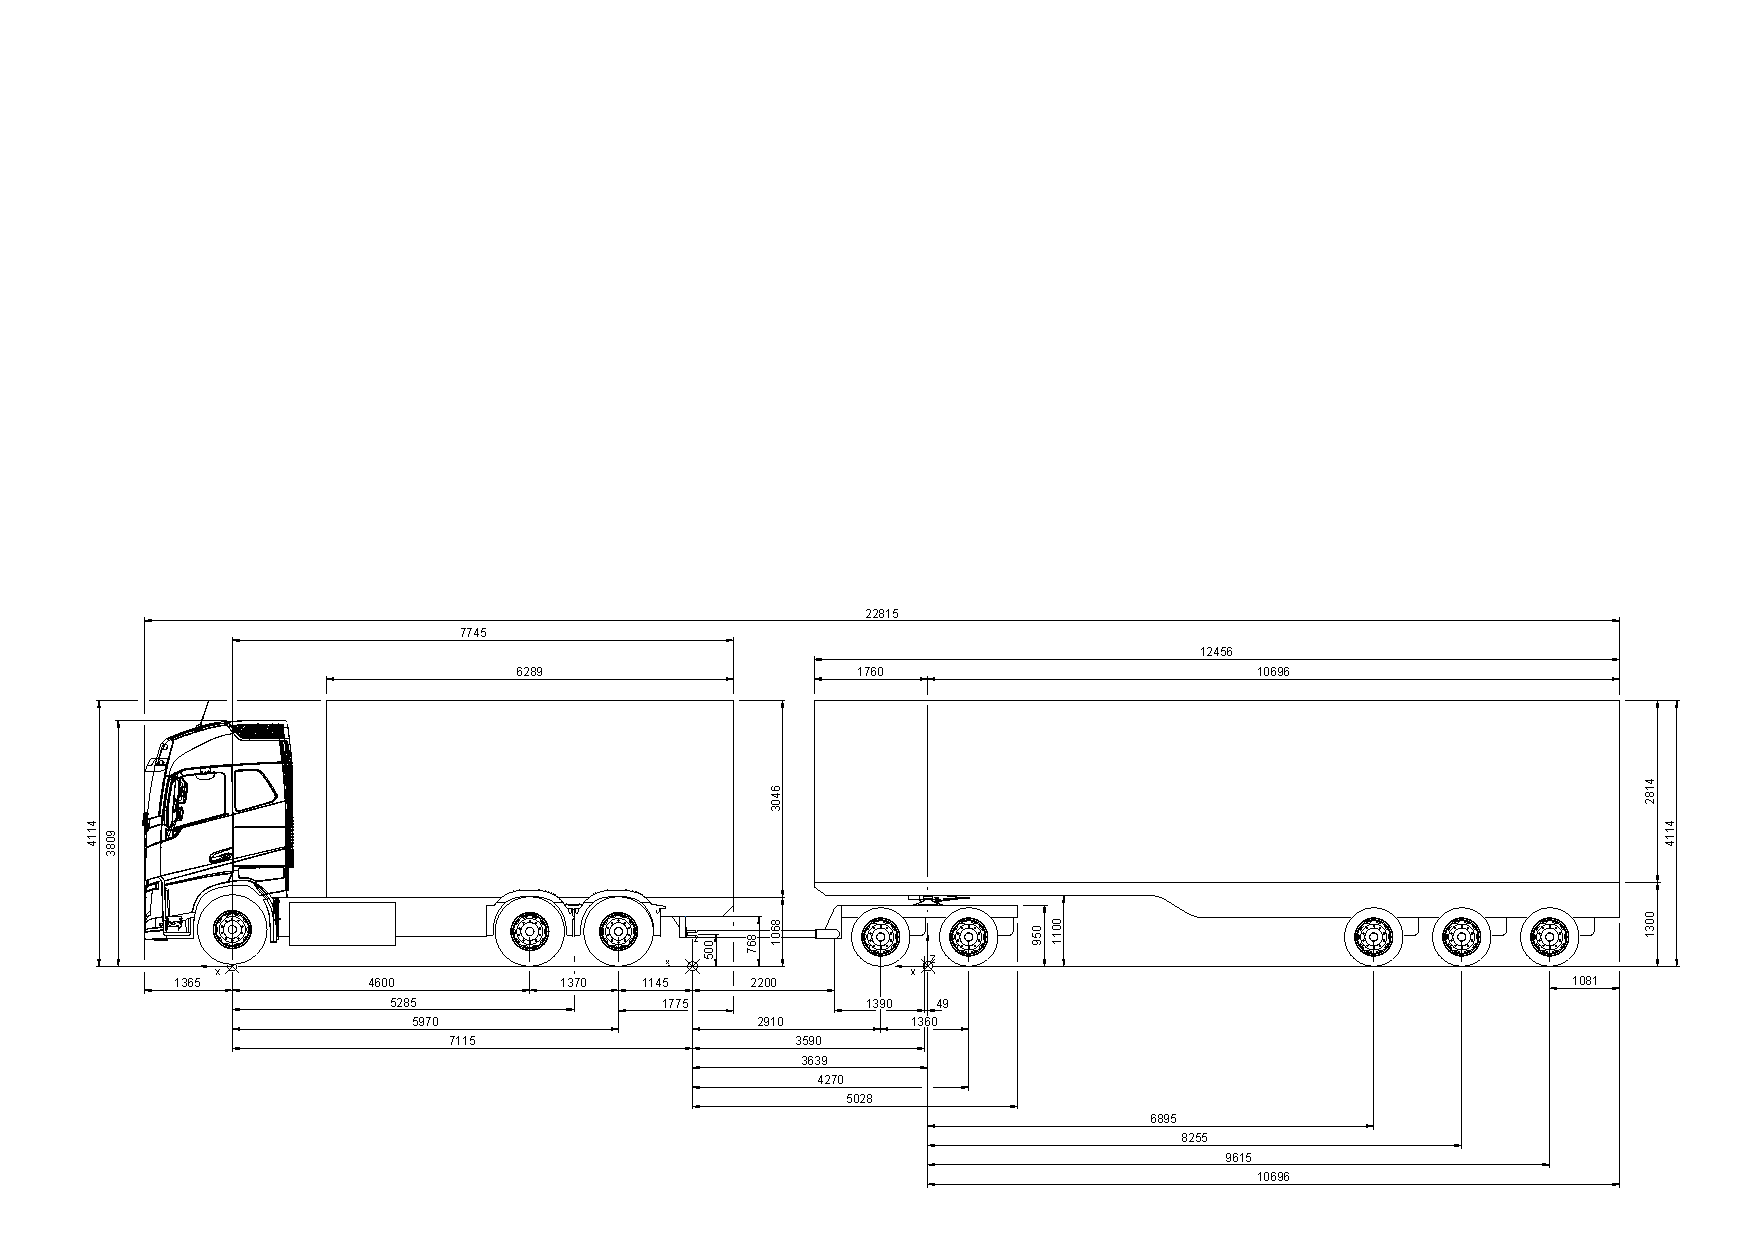
\includegraphics[width=1.3\textwidth]{fig/baseline_ga_rigid-drawbar}
	\caption{Baseline rigid drawbar combination GA drawing}
	\label{figure:baseline-ga-rigid-drawbar-combination}
\end{figure}
%----------------------------------------------
%      FIGURE
%----------------------------------------------
	\vfill
\end{landscape}

\restoregeometry